\section{Технический проект}
\subsection{Технические детали}
Язык программирования: Проект написан на языке программирования Python.

Библиотеки: Проект использует библиотеку SDL2 для графики и обработки событий.

Модули и классы: В коде проекта определены следующие модули и классы:
1. graph-engine:
Функции:создание и настройка графического окна, отрисовка и удаление спрайтов, обработка нажатий на клафиши.
Классы:Graphics: Инициализирует графическое окно, загружает изображения спрайтов, отрисовывает спрайты на экране, обрабатывает события SDL, и завершает работу графической подсистемы SDL.
2. level:
Классы:
Level: Хранит данные об уровне, имеет методы для создания и заполнения уровня тайлами.
LevelAllBricks: Наследуется от Level, определяет конкретный уровень, заполненный одним типом тайлов.
LevelCoridor: Наследуется от LevelAllBricks, определяет уровень с проходом (коридором) из тайлов.
3. the-world:
Классы:
World: Предоставляет функциональность для управления игровыми объектами, добавления/удаления объектов, их обновления и получения информации о них.
4. game-object:
Классы:
GameObject: Определяет базовый игровой объект, его позицию и скорость обновления.
Основной файл main.py:
Импортирует необходимые модули и классы.
Создает экземпляр игры Montezuma и запускает ее.

\subsection{Структура проекта}

\begin{figure}[H]
\centering
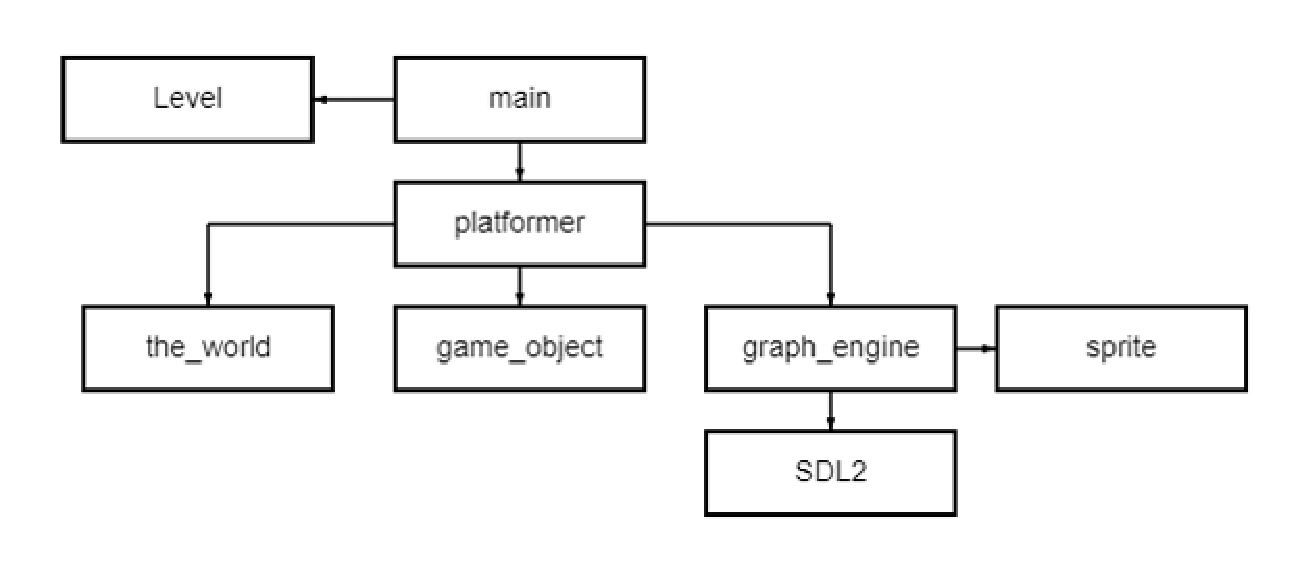
\includegraphics[width=1.05\linewidth]{images/dig1}
\caption{Структура программы}
\label{fig:dig1}
\end{figure}

\begin{figure}[H]
	\center{\includegraphics[width=1.0\linewidth]{UMLMontezuma}}
	\caption{Диаграмма классов}
	\label{UMLMontezuma:image}
\end{figure}

Главный файл main.py: В этом файле вызываются все необходимые модули.

Модуль graph-engine: Модуль для создания и настройки графического окна, создание и отрисовку спрайтоа.

Модуль platformer: Инициализирует графику и запускает игровой цикл.

Модуль the-world: Управляет игровыми объектами, их обновлением и изменением их состояния.

Модуль gameobject: Содержит базовый класс для игровых объектов, определяет их позицию, скорость и обновление.

Модуль sprite: Содержит базовый класс для спрайтов, определяет их позицию и их изображение.

Модуль level: Содержит конфигурацию игровых уровней. 

RESOURCES - объект, предоставляющий доступ к ресурсам (изображениям).

Папка Images: В этой папке содержатся изображения, используемые в игре (например, изображения фона, блоков и персонажа).